\documentclass[11pt]{article}
\usepackage{graphicx}
\usepackage{fancyhdr}
\usepackage{multicol}
\usepackage{listings}
\usepackage[margin=1in]{geometry}
\usepackage[colorlinks=true, linkcolor=black, urlcolor=cyan]{hyperref}

\begin{document}

\begin{titlepage}
\begin{center}
%\includegraphics[height=3.5cm]{images/Standard_CUAUV.jpg}\\[0.2cm]
\textsl{\huge MIT Splash}\\[0.5cm]
{\huge Fall 2014}\\[0.2cm]
\rule{\linewidth}{0.5mm}\\[0.2cm]
{\Huge Machine Learning and Audio Analysis with Python}
\rule{\linewidth}{0.5mm}\\[0.4cm]
\huge Course Notes\\[0.2cm]
\large Daryl Sew
\begin{figure}[h!]
    \centering
        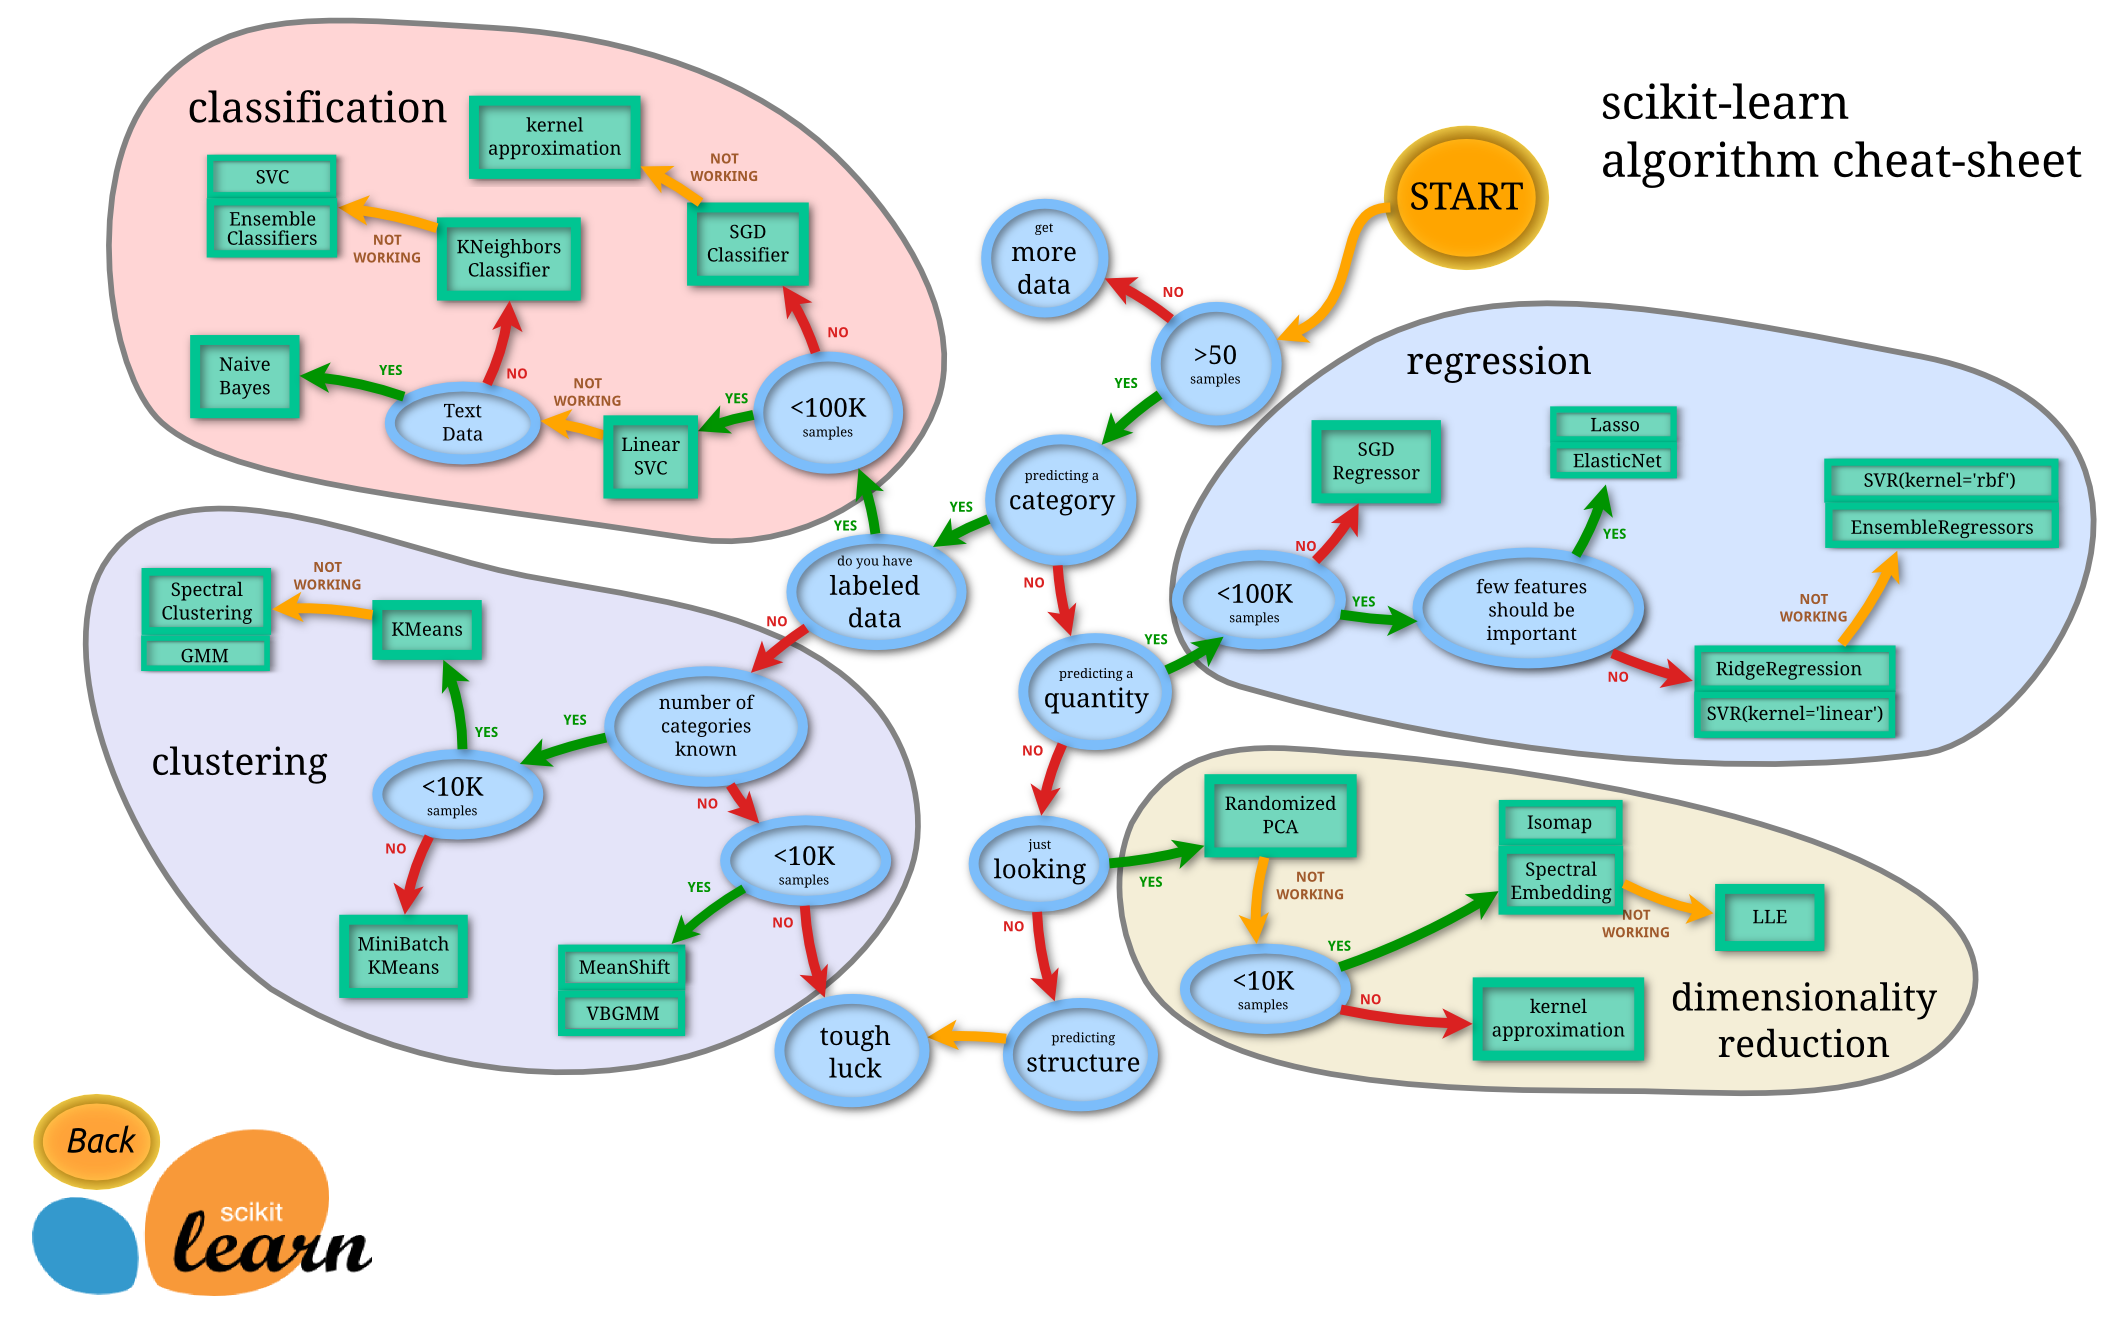
\includegraphics[scale=0.13]{ml_map.png}
        \caption{Flow chart for selecting the right class of algorithm for your problem from \texttt{scikit-learn} }
\end{figure}
\end{center}
\end{titlepage}

% set up header and footer
\pagestyle{fancy}
\fancyhf{}
\setlength{\headheight}{30pt}
\renewcommand{\headrulewidth}{0.4pt}
\renewcommand{\footrulewidth}{0.4pt}
\rhead{Machine Learning and Audio Analysis with Python}

\rfoot{Fall 2014}
\cfoot{\thepage}

% Table of contents
\tableofcontents
\pagebreak

\section{Overview}

Machine learning is a field of computer science that concerns writing programs that can make and improve predictions or behaviors based on data inputs. The applications of machine learning are very diverse - they range from self driving cars to spam filters to autocorrect algorithms and much more. Using scikit-learn, an open source machine learning library for Python, we'll cover reinforcement learning (the kind used to create artificial intelligence for games like chess), supervised learning (the kind used in handwriting recognition), and unsupervised learning (the kind eBay uses to group its products). We'll then cover audio analysis through Fourier transforms with numpy, an open source general purpose computational library for Python, and we'll use our newfound audio analysis and machine learning skills to write very basic speech recognition software. Applications of machine learning to the fields of multitouch gesture recognition and computer vision will also be discussed, drawing from my work at Tesla and research on self driving cars and autonomous submarines.


\section{What is Machine Learning?}
All machine learning algorithms aim to take observations from a system and produce a model of that system. The key words here are 'system' and 'model'. Systems include anything from stock markets to populations of organisms to the environment surrounding a robot, essentially anything imaginable for which you can record observations. Models are a set of mathematical rules that describe a system. Note that in the process of making observations about a system, there will almost always be measurement error - we refer to this as noise, and a good data scientist is able to apply machine learning algorithms in a way that extracts regularities from observations and models those rather than modeling noise.
\subsection{A Brief, Vague History}
The first computer programs were based on explicit instructions; if this, then that. This type of programming is well suited to many tasks, but by no means could these programs be considered 'intelligent' - they were deterministic and could only react to whatever situations their programmer had manually prepared them for. One of the first intelligent programs was written by Arthur Samuel at IBM in 1952 - he applied reinforcement learning to the game of checkers in order to create a model that ranked playing strategies. With this 
\subsection{Motivation}
Knowledge of machine learning and statistical problem solving methods is helpful in a large variety of STEM fields, and it's also in my opinion one of the coolest subfields of computer science.

\section{Unsupervised Learning}
\subsection{K-means clustering}
\subsubsection{Theory}
\subsubsection{Applications}
1-2 examples w code

\section{Semi-supervised Learning}

\section{Supervised Learning}
\subsection{Regression}
Regression is useful for creating a continuous model of a system based on inputs and outputs.
\subsubsection{Theory}
The derivation for linear regression is actually fairly straightforward.
\subsubsection{Applications}

\subsection{Support Vector Machines}
\subsubsection{Theory}
\subsubsection{Applications}
-gesture recognition

\section{Reinforcement Learning}
\subsection{Theory}
-general reinforcement learning
-theory behind neural networks
\subsubsection{Applications}
box2d.js
auv proj (link to RISE based control)

\section{Common Pitfalls}
\subsection{Sampling Bias}
\subsection{Overfitting}
Occam's razor. Polynomial overfitting (a la Wikipedia); using a four layer neural network to model hurricanes; fitting to training set data instead of real data.
One solution is stratified k folding - splitting data into a training set and a testing set.

\section{Algorithm Design Exercises}
Let's see if we can apply these techniques to a novel problem. Note that, as with many problems within data science/machine learning, there isn't necessarily a 'best' way to solve the following problem, as many different methods can arrive at models that are equally good.
\subsection{Pokemon}
You've been tasked with building an AI for Pokemon from scratch. At a high level, how would you go about doing this? You have unlimited time and resources. 
Let's say you're not starting from scratch, and you've been provided with data about every Pokemon Showdown match ever. How does this change your approach?

\section{What is Audio?}

\end{document}
